\section{Generalidades de la Interfaz de OpenERP}
La plataforma OpenERP maneja una interfaz de usuario con unos elementos comunes que permiten mantener una visualización uniforme de todos los módulos a lo largo del sistema, esto permite un fácil aprendizaje de nuevas funcionalidades en la plataforma a través del uso de componentes visuales comunes. En la fígura \ref{fig:enviroment}, puede encontrar:
\begin{itemize}
 \item Manejo del usuario: Permite el cambio de las preferencias de usuario (ej. contraseña, idioma de la interfaz, entre otros)
 \item Accesos rápidos: Permite un rápido a funcionalidades más usadas dentro del sistema
 \item Barra de navegación: Despliega el menú de acceso a los diferentes módulos y funcionalidades disponibles en el sistema
 \item Menú de navegación: Presenta en forma de árbol las opciones de la barra de navegación
 \item Menú contextual: Este menú despliega funciones disponibles basadas en el módulo que se encuentre abierto
\end{itemize}

\begin{figure}[H]
 \centering
 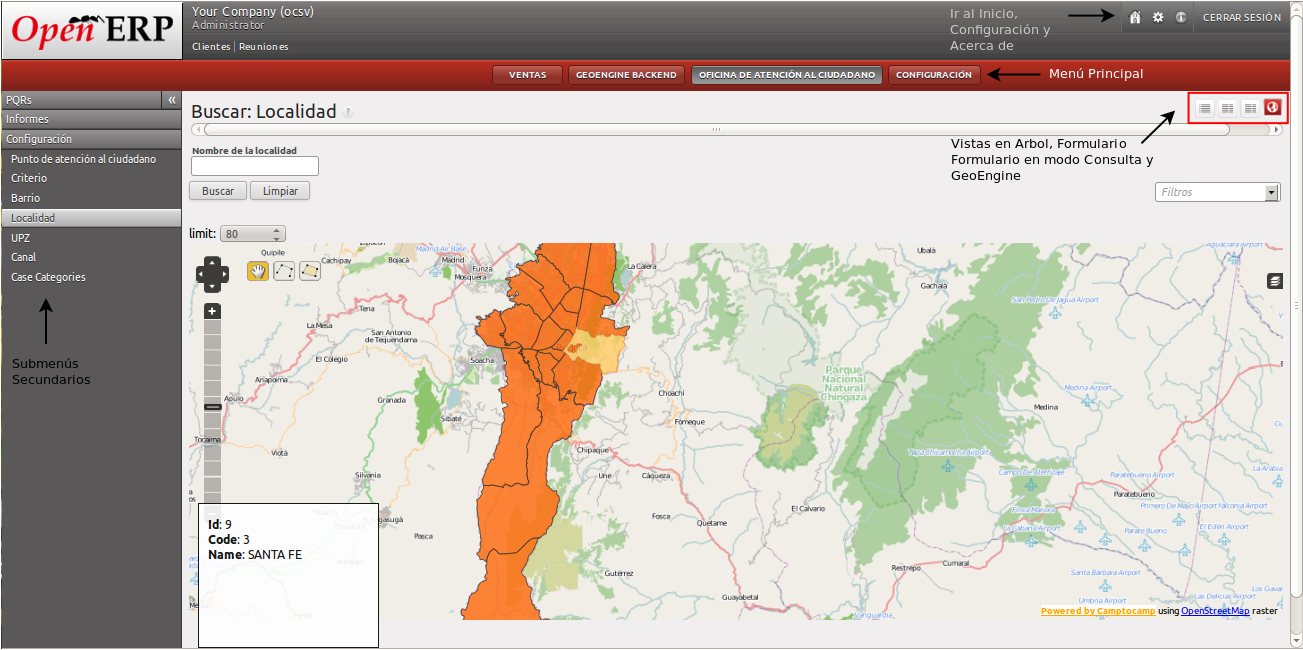
\includegraphics[width=17cm,height=8cm]{./Imagenes/enviroment.png}
 % Login.png: 1289x610 pixel, 96dpi, 34.10x16.14 cm, bb=0 0 967 457
 \caption{Panorama General de OpenERP}
 \label{fig:enviroment}
\end{figure}

\subsection {Cambiar contraseña y cambiar configuración de Idioma}
\begin{itemize}
 \item Hacer clic en el botón \textbf{Configuración}, que tiene forma de rueda dentada y se encuentra en la 
 superior derecha, a la izquierda del botón \textbf{Cerrar Cesión} (Ver figura \ref{fig:enviroment}).
 \item Se despliega una ventana emergente con las opciones de configuración (figura \ref{fig:configuracion}).
 \item En la parte inferior se encuentra el botón  \textbf{Cambiar Contraseña}.
 \item En la parte media de la ventana se encuentran los idiomas disponibles para la aplicación, por defecto
 se encuentra el Inglés y el Idioma Local (Spanish-CO). 
\end{itemize}

\begin{figure}[H]
 \centering
 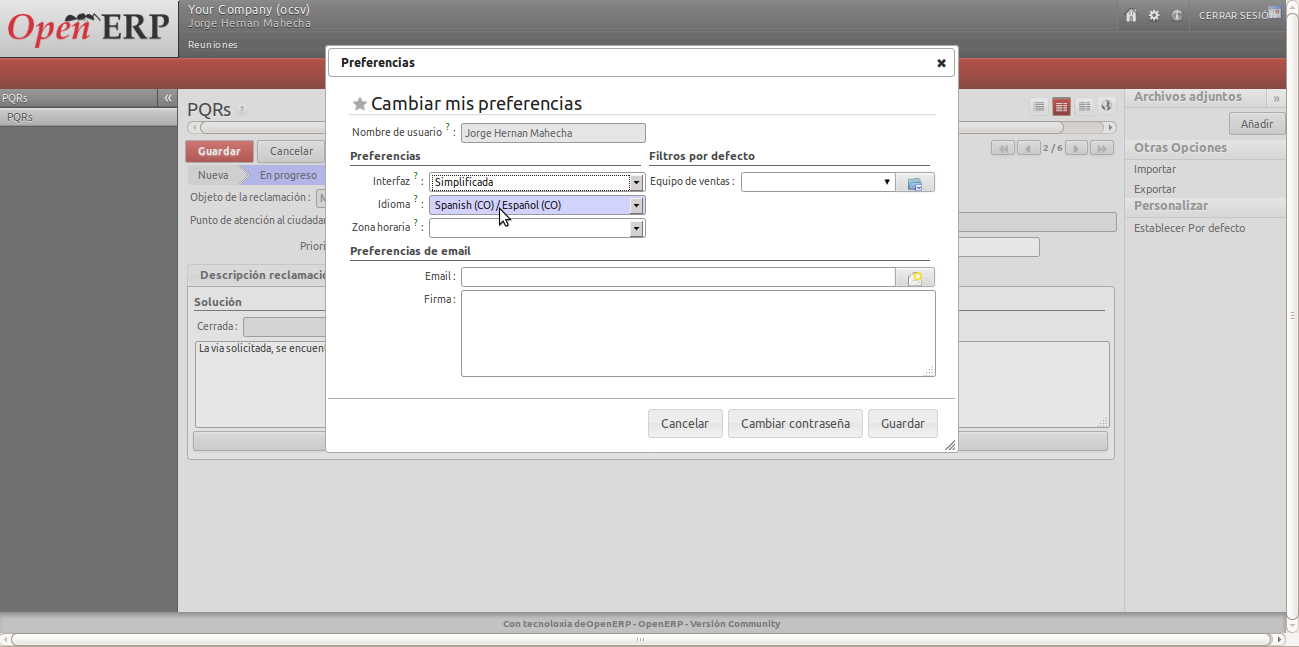
\includegraphics[width=17cm,height=8cm]{./Imagenes/configuracion.png}
 % Login.png: 1289x610 pixel, 96dpi, 34.10x16.14 cm, bb=0 0 967 457
 \caption{Ventana de configuración de preferencias y cambio de contraseña}
 \label{fig:configuracion}
\end{figure}


\subsection{Tipos de Vistas}
Existen en OpenERP varios tipos de vistas, que nos permiten ver la información disponible en el sistema en diversas maneras:
\begin{itemize}
 \item Lista, despliega todos los registros de información disponibles para el módulo abierto .
 \item Formulario, permite la edición de un registro disponible en el sistema.
 \item Geográfica (GeoEngine), permite la visualización de los registros del sistema ubicados en un mapa.
 \item Kanban, despliega la información en forma de tarjetas en un tablero.
 \item Gantt, despliega información en un diagrama de Gantt.
 \item Calendario, presenta la información en un calendario en vista mensual.
 \item Gráfico, despliega información resumida en diagrama de barras.
\end{itemize}
Las vistas disponibles para una aplicación se encuentran en la parte superior derecha, debajo de la barra del menú de navegación (Ver \ref{fig:barravistas}).
Para pasar de una vista a otra simplemente se hace clic en el icono correspondiente. El listado de vistas disponibles varia de módulo a módulo.
\begin{figure}[H]
 \centering
 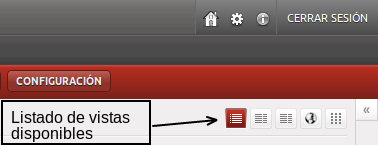
\includegraphics[width=10cm,height=3cm]{./Imagenes/barravistas.png}
 % Login.png: 1289x610 pixel, 96dpi, 34.10x16.14 cm, bb=0 0 967 457
 \caption{Íconos para el cambio de vistas}
 \label{fig:barravistas}
\end{figure}

\subsection{Elementos en la vista tipo lista}
\begin{itemize}
 \item \textbf{Filtro de datos}: En la vista tipo lista se encuentran botones para filtrar y agrupar los registros disponibles en el módulo (Ver figura \ref{fig:filtro}), solo debe hacer clic en los diferentes iconos disponibles.
  \begin{figure}[H]
  \centering
  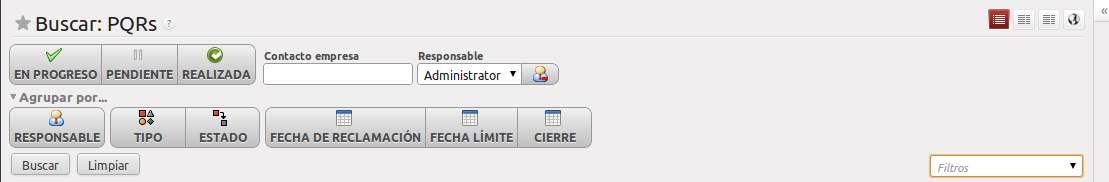
\includegraphics[width=15cm,height=3cm]{./Imagenes/filtro.png}
    \caption{Iconos para filtrar y agrupar registros}
  \label{fig:filtro}
  \end{figure}

 \item \textbf{Listado de registros}: El objetivo principal de esta vista es la de listar los registros almacenados en el módulo, existen varias opciones para el manejo de dichos registros, generalmente se encuentran:
 \begin{itemize}
 \item \textbf{crear un nuevo registro}: haciendo clic en el botón de crear se despliega un formulario para crear un nuevo registro.
 \item \textbf{borrar un registro}: haga clic en el botón de chequeo de los registros que desea eliminar y luego haga clic en el botón para borrar los registros seleccionados.
 \item \textbf{editar registros}: haciendo clic en el ícono del lápiz se despliega el formulario para editar el registro seleccionados.
 \item \textbf{ver detalle}: haciendo clic en cualquier parte del registro se despliegan todos los detalles del registro seleccionado en modo de solo lectura.
 \item \textbf{paginador}: el modo de lista despliega un número limitado de registros, usted puede ver las páginas que contienen los otros registros no listados haciendo uso del los botones disponibles en el paginador.
 \end{itemize}
  \begin{figure}[H]
  \centering
  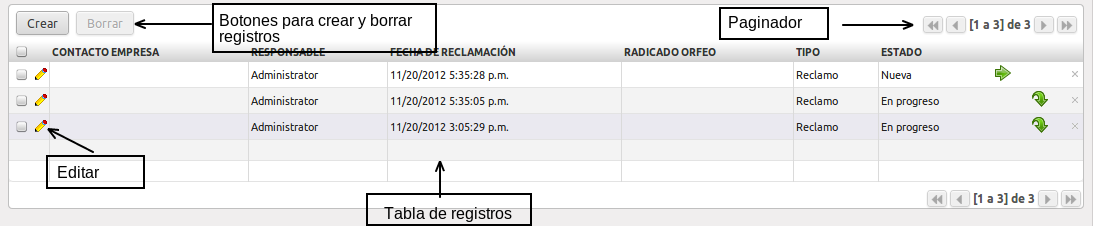
\includegraphics[width=17cm,height=5cm]{./Imagenes/listadoregistros.png}
    \caption{Listado de registros}
  \label{fig:listadoregistros}
  \end{figure}

\end{itemize}


\subsection{Iconos Comúnes en la vista de formulario}
\begin{enumerate}
 \item \textbf{Barra de Estados} 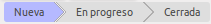
\includegraphics[width=4cm,height=0.5cm]{./Imagenes/barraestados.png}:
  Muchos de los objetos que conforman OpenERP cambian de estado de acuerdo de acuerdo a como se desarrolla el
  flujo de trabajo. La barra de estado muestra como va cada proceso que se está llevando a cabo, su ubicación es variable
  y generalmente el estado actual de un proceso está demarcado con un color diferente.
 \item \textbf {Icono de entidades relacionadas} 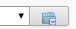
\includegraphics[width=2cm,height=0.7cm]{./Imagenes/entidadesrelacionadas.png}: Cuando un campo tiene este icono al lado,
 significa que se está relacionando otra entidad dentro de la aplicación, por ejemplo cuando se menciona una empresa o un contacto, se está mostrando la información una entidad
 de empresas o una entidad de contactos. El ícono significa además que se puede  \textbf{crear}, \textbf{editar} o \textbf{buscar} un registro para insertarlo en el campo. 
 Sin embargo estas opciones estarán disponibles para el usuario de acuerdo con su perfil, los permisos están clasificados para leer, modificar, crear
 o eliminar un registro dentro de una entidad específica. 
 \item \textbf {Icono de ayuda}: Este se identifica por el símbolo de interrogación '?', al posicionar el puntero del ratón sobre este ícono se despliega información de ayuda acerca del campo del formulario.
\end{enumerate}

\subsection{Ingreso al Sistema}
\begin{figure}[H]
 \centering
 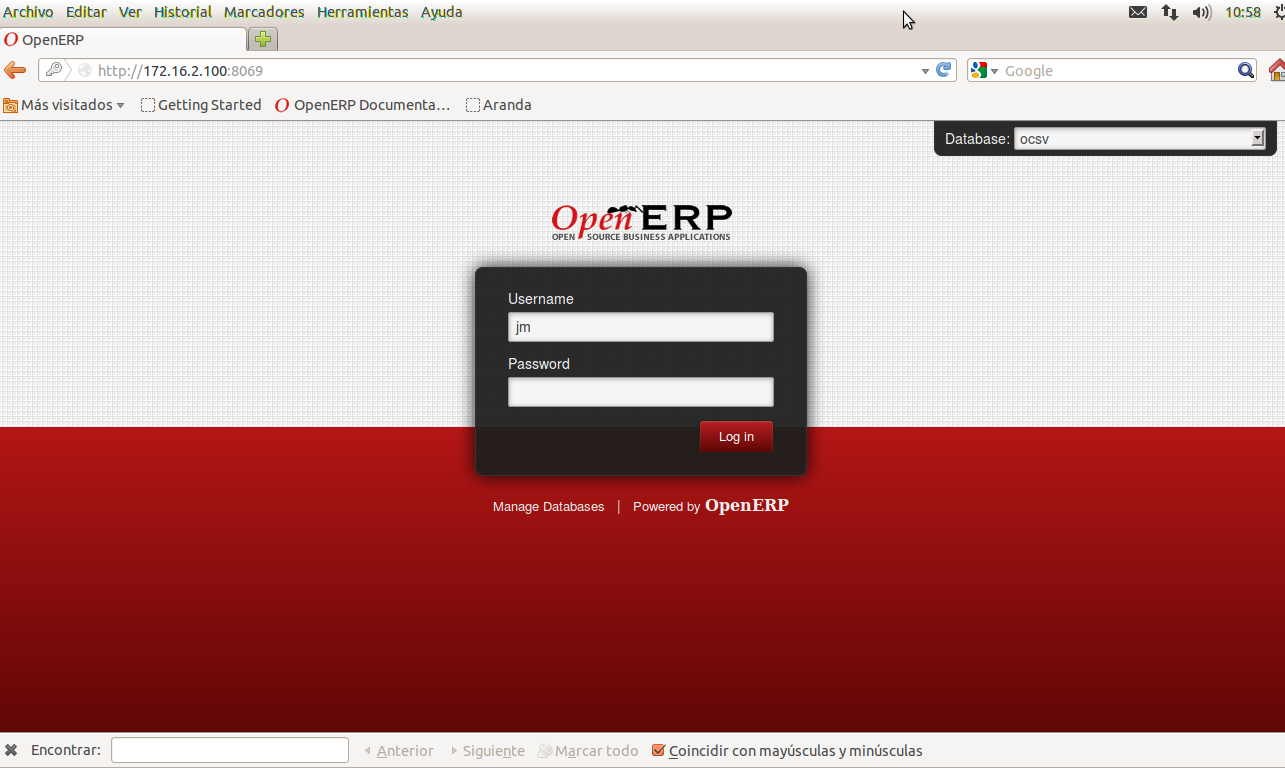
\includegraphics[width=17cm,height=10cm]{./Imagenes/Login.png}
 % Login.png: 1289x610 pixel, 96dpi, 34.10x16.14 cm, bb=0 0 967 457
 \caption{Pantalla de Inicio}
 \label{fig:login}
\end{figure}


\begin{itemize}
 \item Para ingresar al sistema utilice un navegador web actualizado y con soporte de javascript activado(se recomienda: Mozilla Firefox o Google Chrome), y en la barra de direcciones coloque la dirección del servidor: ej \underline{http://openerp.idu.gov.co}. Aparecerá la pantalla
 de inicio que se ve en la figura \ref{fig:login}
 \item Ingrese los datos de su cuenta, nombre de usuario y clave.
 \item Si los datos de la cuenta son correctos, la siguiente pantalla muestra el menú principal de la aplicación (ver: \ref{fig:menumain}).
\end{itemize}


\begin{figure}[H]
 \centering
 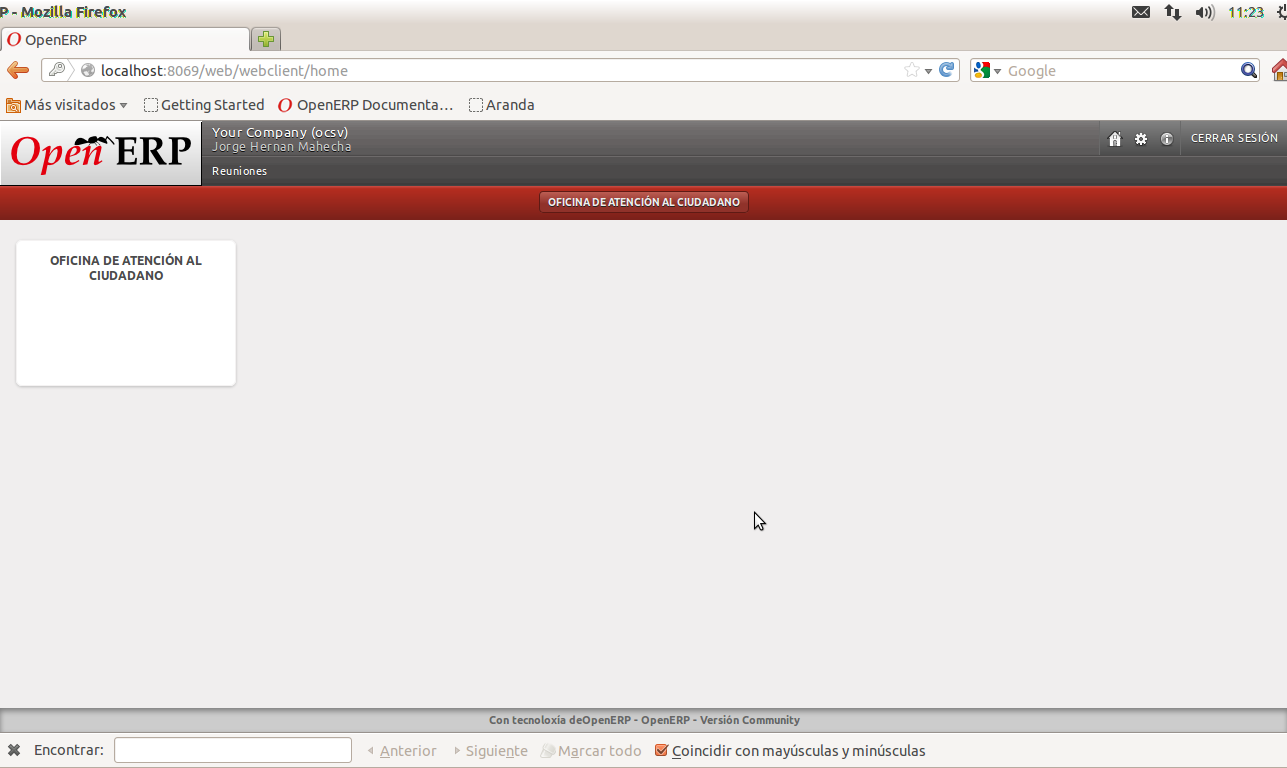
\includegraphics[width=17cm,height=10cm]{./Imagenes/menumain.png}
 % Login.png: 1289x610 pixel, 96dpi, 34.10x16.14 cm, bb=0 0 967 457
 \caption{Menú Principal de la aplicación}
 \label{fig:menumain}
\end{figure}
